%---------------------------------------------------------------------------%
%->> Chapter 4: 故障诊断智能体平台设计与实现
%---------------------------------------------------------------------------%

\chapter{故障诊断智能体平台设计与实现}

第三章提出了故障指纹构建、SOP自动化构建以及 SOP 驱动的智能体在线故障诊断方法。本章在此基础上，进一步介绍故障诊断智能体平台的设计与实现，重点说明上述方法在系统中的落地方式。围绕平台对离线知识构建与在线故障诊断两类任务的支撑，本文将从平台总体架构、关键功能实现、任务执行与数据管理机制以及主要交互界面等方面展开说明，以展示方法设计与平台实现之间的对应关系。

%---------------------------------------------------------------------------%
%->> 4.1 平台架构
%---------------------------------------------------------------------------%
%---------------%
%->> Section 4.1: 系统架构
%------------%

\section{系统架构}

微服务故障诊断并不是固定流程下的顺序执行任务，而是一个由中间证据持续驱动的动态决策过程。任务开始时，系统通常只能获得告警信息、异常服务以及少量上下文；在后续诊断过程中，应优先检查哪些指标、日志或链路对象，是否继续沿当前路径深入，以及何时停止当前分支并转向其他可疑组件，都需要根据不断获得的新证据实时调整。与此同时，诊断过程还伴随着文件访问、命令执行、工具调用、状态记录和多轮任务推进等操作。因此，支撑该任务的平台不仅需要具备智能体运行能力，还需要提供面向工程环境的执行能力，以支持“边观察、边判断、边调整”的诊断过程。

基于上述特点，本文采用 OpenCode 作为故障诊断智能体平台的运行基础，而未将系统建立在传统智能体框架之上。一方面，OpenCode 作为开源平台，系统结构与执行链路较为透明，便于功能扩展、本地部署和实验复现；另一方面，OpenCode 原生支持多模型提供商与本地模型接入，可根据成本、时延和能力需求灵活切换模型。更重要的是，OpenCode 提供了 agent、subagent、skill、custom command 和 MCP server 等机制~\cite{opencode2025,claudecode_skills,mcp,luo2025mcpuniverse}，能够较好覆盖本文在任务拆分、角色分工、工具接入与执行控制等方面的实现需求。同时，其运行环境天然支持文件操作、命令执行和外部工具调用，更适合承载微服务故障诊断这类工具密集、路径动态变化的任务。

平台总体架构如图\ref{fig:system_architecture}所示。系统自上而下划分为前端展示层、Agent 执行层、Skill 组织层、MCP 接入层、后端服务层、数据存储层和外部服务层。前端展示层提供 Web 界面、SOP 可视化、故障指纹视图、诊断结果展示以及实时通信能力，用于支撑用户交互和任务状态反馈；Agent 执行层负责维护会话、加载 Skill、创建子代理并推进任务执行；Skill 组织层封装在线诊断、离线探索和规则整理三类核心任务；MCP 接入层将后端接口和观测能力以统一工具形式暴露给 Agent；后端服务层提供诊断任务 API、SOP 管理 API、故障指纹管理 API 以及数据查询 API；数据存储层保存 SOP 知识库、故障指纹库、执行轨迹和实验数据；外部服务层则负责提供大语言模型服务与监控数据源。各层通过标准接口衔接，形成了从前端交互、任务执行到结果持久化的完整链路。

\begin{figure}[htbp]
    \centering
    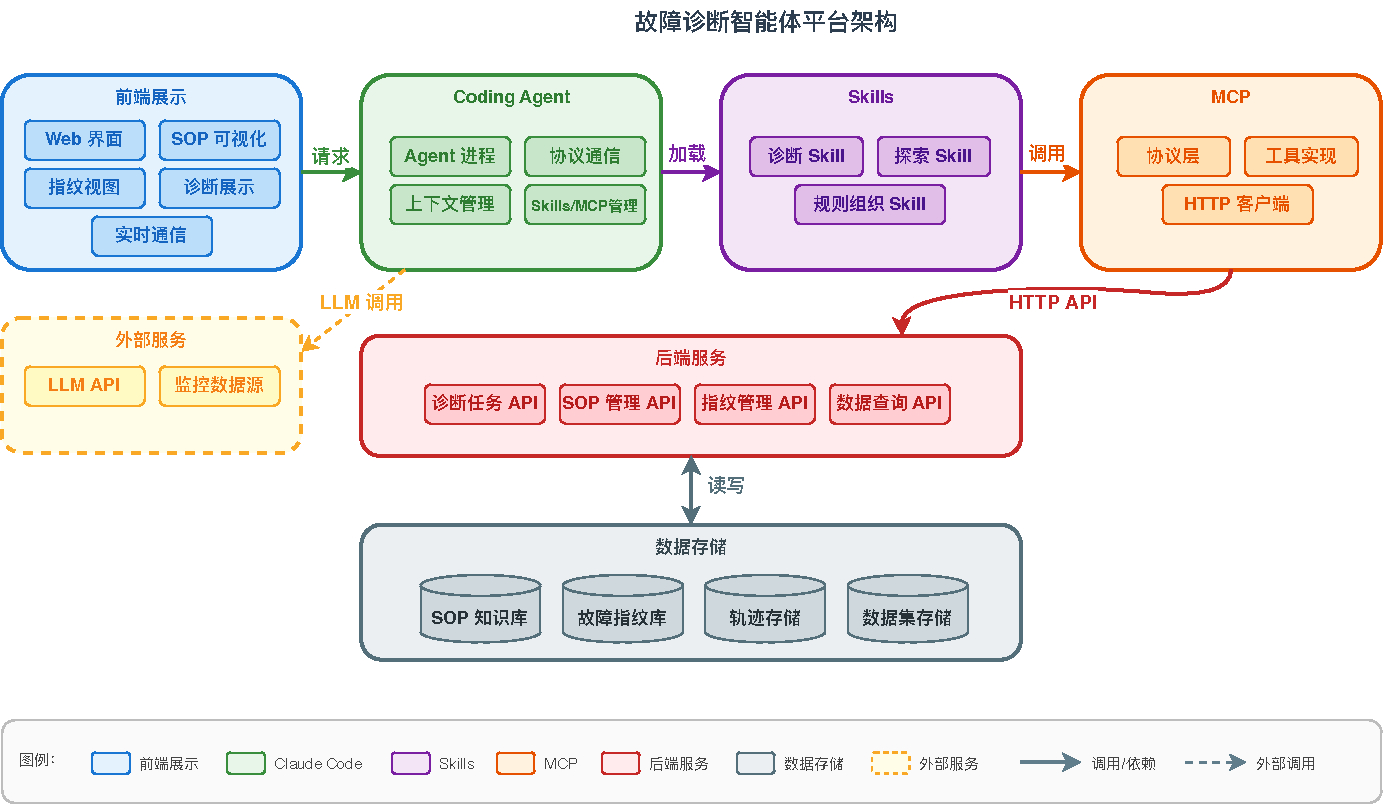
\includegraphics[width=\textwidth]{Figures-Src/Chap4-System/system-architecture/chart.pdf}
    \bicaption{基于 OpenCode 的微服务故障诊断平台架构}{Architecture of the Microservice Fault Diagnosis Platform Based on OpenCode}
    \label{fig:system_architecture}
\end{figure}

围绕第三章提出的方法，平台将系统中的核心任务进一步组织为 \texttt{Diagnosis-Skill}、\texttt{Exploration-Skill} 和 \texttt{Rule-Skill} 三类 Skill。其中，\texttt{Diagnosis-Skill} 面向告警驱动的在线诊断任务，负责读取告警信息、故障指纹检索结果和当前 SOP，并输出诊断结论与执行记录；\texttt{Exploration-Skill} 面向离线知识构建中的探索任务，围绕场景先验、可疑对象和现有 SOP 生成探索轨迹与补充证据；\texttt{Rule-Skill} 面向规则整理任务，读取探索轨迹与历史诊断记录，输出决策单元及更新后的 SOP。通过这种拆分方式，每个会话只加载与当前任务直接相关的约束、工具和上下文，从而避免不同任务逻辑在同一会话中相互干扰。

在平台中，Skill 用于组织任务目标与执行约束~\cite{claudecode_skills,claudecode-subagent}，MCP 用于接入具体能力~\cite{mcp,luo2025mcpuniverse,jayanti2026camcp,koc2025mcpide}。前者定义任务的输入输出形式、执行边界与行为规则，后者负责将后端接口和数据查询能力暴露为 Agent 可调用的统一工具。围绕这一分工，平台设置了 \texttt{Diagnosis MCP}、\texttt{Exploration MCP}、\texttt{Rule MCP} 和 \texttt{Observe MCP} 四类 MCP。其中，前三者分别服务于三类主任务，封装对应的操作说明、接口定义和结果返回方式；\texttt{Observe MCP} 则统一提供指标、日志、链路和感知域相关的查询能力。

指标查询、日志检索、链路分析以及感知域补充并未被进一步封装为独立的主 Skill，而是作为共享观测能力由各主任务按需调用。为此，平台引入观察子代理（Observe subagent）~\cite{claudecode-subagent}。当 \texttt{Diagnosis-Skill} 或 \texttt{Exploration-Skill} 在执行过程中需要补充观测证据时，主会话首先创建观察子代理，再由后者通过 \texttt{Observe MCP} 完成专项查询。主会话负责诊断推进、路径选择与状态维护，观察子代理负责围绕指定对象采集证据并返回结果。这样的组织方式不仅能够控制主会话的上下文规模，也使流程控制与证据采集相互分离，便于后续扩展新的观测能力。

从任务执行角度看，平台运行过程可概括为三个阶段。首先，用户通过前端发起在线诊断或离线知识构建请求，后端据此创建对应工作区并初始化场景上下文。其次，OpenCode 根据任务类型启动相应会话并加载对应 Skill：在线任务加载 \texttt{Diagnosis-Skill}，离线探索任务加载 \texttt{Exploration-Skill}，规则整理任务加载 \texttt{Rule-Skill}。最后，主 Skill 在运行过程中通过 MCP 调用后端接口；当需要补充观测证据时，再创建观察子代理，由其通过 \texttt{Observe MCP} 完成专项查询。执行过程中产生的轨迹、状态与结果持续同步至后端与数据存储层，并通过实时通信反馈到前端界面。经人工确认后的有效案例进一步回流至故障指纹库和 SOP 知识库，为后续离线更新提供输入，从而形成在线执行、结果沉淀与知识更新的闭环。

综上，本文基于 OpenCode 实现了面向微服务根因定位的故障诊断智能体平台。该平台以 Skill 承担在线诊断、离线探索和规则整理三类主任务，以 MCP 连接后端能力与观测工具，并通过观察子代理完成专项证据采集。整体架构能够适应微服务故障诊断中路径动态、工具密集和知识持续更新的任务特点，为后续在线诊断与离线知识演化提供统一的平台支撑。

%---------------------------------------------------------------------------%
%->> 4.2 系统实现
%---------------------------------------------------------------------------%
%--------------%
%->> Section 4.2: 系统实现
%------------%

\section{系统实现}

本节进一步说明第三章提出的三类方法在平台中的具体落地方式。围绕故障指纹构建、SOP自动化构建和在线故障诊断三类核心方法，平台分别形成了对应的实现链路。表\ref{tab:chap3_chap4_impl}给出了第三章方法与平台实现之间的对应关系。

\begin{table}[htbp]
    \centering
    \bicaption{\enspace 第三章方法与平台实现的对应关系}{\enspace Mapping of Chapter 3 Methods to Platform Components}
    \label{tab:chap3_chap4_impl}
    \begingroup
    \small
    \setlength{\tabcolsep}{4pt}
    \renewcommand{\arraystretch}{1.25}
    \begin{tabularx}{\textwidth}{>{\raggedright\arraybackslash}p{3.3cm}>{\raggedright\arraybackslash}p{4.0cm}>{\raggedright\arraybackslash}X}
        \toprule
        \textbf{第三章方法} & \textbf{平台中的主要位置} & \textbf{具体实现} \\
        \midrule
        故障指纹构建方法 & 故障指纹库、指纹管理模块、编码模型服务 & 负责故障指纹编码、存储、聚类维护和在线检索，并返回相似故障及其绑定的SOP \\
        SOP 自动化构建方法 & 工作区、\texttt{Exploration-Skill}、\texttt{Rule-Skill}、轨迹存储 & 负责生成探索轨迹、提取决策单元，并完成SOP更新 \\
        在线故障诊断方法 & \texttt{Diagnosis-Skill}、观察 subagent、结果回流更新机制 & 负责读取告警与SOP、收集证据、推进诊断，并将结果回流至后续更新流程 \\
        \bottomrule
    \end{tabularx}
    \endgroup
\end{table}

\subsection{故障指纹构建方法的实现}

第 3.2 节提出的传播感知多模态故障指纹构建方法，主要由故障指纹库、指纹管理模块和编码模型服务共同实现。由于该部分任务以批处理和持续维护为主，涉及特征编码、向量存储与聚类更新，因此其核心计算逻辑部署在后端服务侧。

在离线阶段，系统首先从历史故障实例中抽取指标、日志和链路等多模态数据，再调用编码模型服务生成 MMF、CTF、LCF、LSF 和 CMF 五类特征，并将其拼接形成故障指纹，存入故障指纹库。除保存指纹向量外，故障指纹库还维护聚类中心以及故障簇与SOP的绑定关系。指纹管理模块负责这些记录的更新，并定期对已有指纹执行DBSCAN聚类，以刷新聚类中心和绑定结果。

在在线阶段，系统接收到告警后，由后端首先调用指纹管理模块完成相似故障检索，返回最近邻故障簇及其绑定的SOP，再将检索结果同步到当前工作区，作为 \texttt{Diagnosis-Skill} 的初始上下文。通过这一实现方式，在线诊断在开始时即可获得与当前告警最接近的历史故障模式及其对应的排查流程。

\subsection{SOP自动化构建方法的实现}

第 3.3 节提出的SOP自动化构建方法，在平台中由 \texttt{Exploration-Skill} 和 \texttt{Rule-Skill} 依次完成。前者负责围绕给定故障场景生成可分析的探索轨迹，后者负责从这些轨迹中提取决策单元并更新 SOP 知识库。之所以将二者分开执行，是因为探索阶段关注证据扩展和路径尝试，而规则阶段关注结构整理与知识沉淀，两类任务在输入、输出和控制目标上均存在明显差异。

在具体实现中，后端首先围绕某一故障实例创建工作区，并初始化故障类型先验、相关服务范围和当前SOP。随后，系统启动多个代理，基于 \texttt{Exploration-Skill} 并行执行故障探索任务，从而生成多条 SOP 执行轨迹。在每个代理的执行过程中，\texttt{Exploration-Skill} 负责约束探索行为，包括下一步检查对象、路径推进方式以及当前探索的结束条件；若某一步需要补充指标、日志或链路证据，则创建观察 subagent，由其通过 \texttt{Observe MCP} 获取所需信息并返回结果。

探索结束后，生成的轨迹被保存至轨迹存储。随后系统启动 \texttt{Rule-Skill}，读取这些轨迹，对其中的关键判断、跳转条件和结论形成过程进行拆解，完成决策单元提取、语义对齐和权重计算。最后，\texttt{Rule-Skill} 根据高权重决策单元对原有 SOP 执行节点的增删改操作，并将更新后的有向图同步至SOP知识库。由此，SOP的更新过程被组织为“探索生成轨迹—规则整理轨迹—知识库完成更新”的连续实现链路。

\subsection{在线故障诊断方法的实现}

第 3.4 节提出的SOP驱动多智能体在线故障诊断方法，主要由 \texttt{Diagnosis-Skill}、观察 subagent 和结果回流更新机制共同实现。系统接收到告警后，后端首先完成两项准备工作：一是调用故障指纹检索接口，获得最近邻故障簇及其绑定的SOP；二是创建工作区，并将告警信息、检索结果和选定的SOP初始化到当前任务上下文中。随后，OpenCode 启动诊断会话，加载 \texttt{Diagnosis-Skill}，并据此初始化焦点与感知域。

诊断开始后，\texttt{Diagnosis-Skill} 负责主流程推进。它根据当前焦点和已有证据决定下一步动作，并在运行过程中执行三类核心操作：\texttt{navigate} 表示沿当前 SOP 继续推进，\texttt{escape} 表示在现有SOP无法覆盖当前场景时通过逃逸机制扩展新的诊断路径，\texttt{conclude} 表示输出当前诊断结论。上述操作由 \texttt{Diagnosis MCP} 提供相应的接口和执行约束。

与离线探索阶段相同，\texttt{Diagnosis-Skill} 并不直接访问指标、日志和链路数据。当诊断过程需要补充某一焦点范围内的可观测证据时，主会话会创建观察 subagent，由后者通过 \texttt{Observe MCP} 查询所需数据，再将结果返回主流程。这样，诊断过程中的路径控制与证据采集被明确分离：前者由主会话负责，后者由观察子代理承担。

诊断结束后，系统将诊断结论、关键证据和完整执行过程保存为候选诊断记录。经过人工审核后，相关结果将进一步进入故障指纹更新流程和SOP增量更新流程，用于补充后续任务所依赖的历史知识。通过这一实现方式，在线诊断不仅能够利用已有知识完成当前故障定位，也能够将新的有效经验持续回流至平台知识体系中。

综上，第三章提出的三类方法在平台中分别落地为故障指纹检索、SOP自动化构建和在线诊断执行三条实现链路。三者侧重点不同，但通过工作区、知识库以及结果回流更新机制连接在一起，共同构成了平台的核心实现流程。

%---------------------------------------------------------------------------%
%->> 4.3 任务执行与数据管理
%---------------------------------------------------------------------------%
%--------%
%->> Section 4.3: 任务执行与数据管理
%------------------%

\section{任务执行与数据管理}

前两节分别说明了平台的总体架构，以及第三章三类方法在系统中的实现方式。本节进一步介绍任务在平台中的组织形式，以及相关数据在执行过程中的管理方式。这里主要涉及两方面内容：其一，工作区、任务与知识库之间的数据关系；其二，离线知识构建任务与在线诊断任务的执行过程。

平台以工作区作为任务运行的基本单元。无论是在线诊断还是离线知识构建，系统都会先创建独立工作区，并在其中初始化该任务所需的故障实例信息、接口地址、当前 SOP 和任务标识等上下文。通过这种方式，一次任务执行过程中涉及的数据、状态与结果都被统一组织在同一工作区之下，从而便于后续管理、复现与结果回流更新。

图\ref{fig:system_data_model}给出了工作区、任务与 SOP 之间的数据关系。

\begin{figure}[htbp]
    \centering
    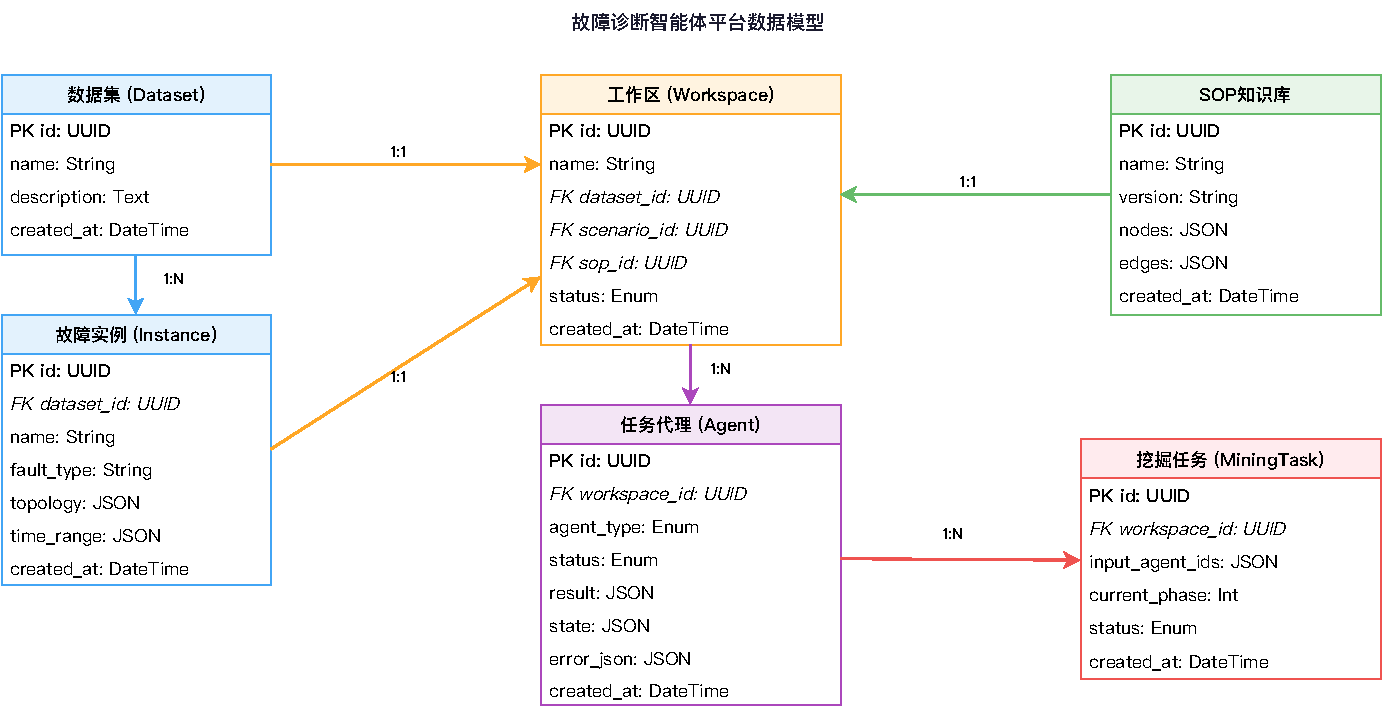
\includegraphics[width=0.92\textwidth]{Figures-Src/Chap4-System/data-model/chart.pdf}
    \bicaption{\enspace 工作区、任务与SOP的数据关系}{\enspace Data Relationships Among Workspaces, Tasks, and SOPs}
    \label{fig:system_data_model}
\end{figure}

如图\ref{fig:system_data_model}所示，系统中的数据模型包含六个核心实体。Dataset（数据集）保存原始数据的基础信息；Instance（故障实例）记录数据集下单次故障的可观测数据及其故障信息，同一数据集可以对应多个故障实例；Workspace（工作区）将数据、故障实例和 SOP 组织到一次任务执行中，并通过外键唯一关联一个数据集、一个故障实例和一个 SOP 知识库；SOP Knowledge Base（SOP 知识库）以有向图形式保存 SOP；Agent（任务代理）记录一次具体任务的执行状态与任务类型；MiningTask（挖掘任务）记录离线规则整理相关任务。通过这一数据结构，同一故障实例可以在在线诊断和离线知识构建两个阶段挂接到统一的工作区上下文下，从而便于共享故障实例信息与历史结果。

从任务组织方式看，平台中的 Agent 可分为两类。第一类是主任务代理，分别加载 \texttt{Diagnosis-Skill}、\texttt{Exploration-Skill} 和 \texttt{Rule-Skill}，负责在线诊断、离线探索和规则整理三类主任务；第二类是观察 subagent，其不承担完整任务流程，仅在主任务需要补充观测数据时被临时创建，用于调用 \texttt{Observe MCP} 执行专项查询。这种划分方式使流程控制与数据采集相互分离，也避免主任务会话长期携带大量观测工具上下文。

离线知识构建任务的执行过程可以概括为以下三个环节：

\begin{enumerate}[label=（\arabic*）]
    \item \textbf{探索轨迹生成。}
    用户在前端发起 SOP 构建任务后，后端首先创建工作区，并启动 \texttt{Exploration-Skill}。在执行过程中，\texttt{Exploration-Skill} 围绕当前 SOP 进行多轮探索，决定每一步应检查的节点以及需要补充的证据；若需要访问指标、日志或链路数据，则创建观察 subagent，由其通过 \texttt{Observe MCP} 完成相应查询。探索过程中形成的判断路径和观测结果会持续保存至轨迹存储。

    \item \textbf{规则整理与决策单元提取。}
    在轨迹生成完成后，后端读取轨迹存储中的探索轨迹，并启动 \texttt{Rule-Skill}。该阶段主要对轨迹中的关键判断、节点跳转和结论形成过程进行拆解，完成语义归一化、决策单元提取与权重计算。第 3 章定义的四项指标 MI、DF、TD 和 EV 也在这一阶段完成计算与聚合。

    \item \textbf{SOP 增量更新。}
    \texttt{Rule-Skill} 根据高权重决策单元对原有 SOP 执行节点增删改操作，并将更新后的有向图同步至 SOP 知识库。任务完成后，系统将构建结果返回前端，从而形成一次完整的离线知识构建流程。
\end{enumerate}

在线故障诊断阶段的执行时序如图\ref{fig:online_sequence}所示，在线诊断过程可以进一步概括为以下五个步骤：


\begin{figure}[htbp]
    \centering
    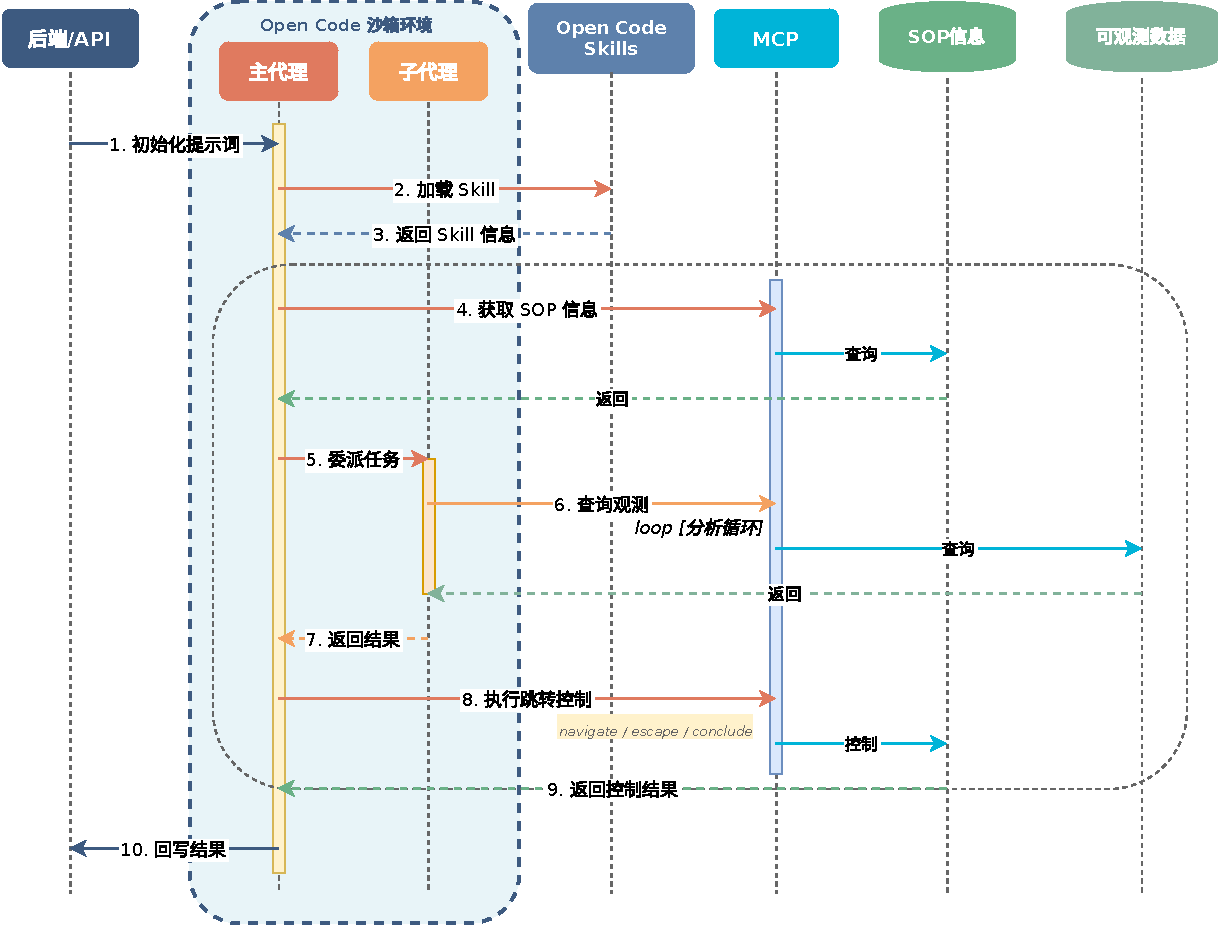
\includegraphics[width=0.98\textwidth]{Figures-Src/Chap4-System/online-diagnosis-timeline/chart.pdf}
    \bicaption{\enspace 在线诊断任务执行时序}{\enspace Execution Sequence of an Online Diagnosis Task}
    \label{fig:online_sequence}
\end{figure}


\begin{enumerate}[label=（\arabic*）]
    \item \textbf{任务初始化。}
    后端接收到告警后，首先完成故障指纹检索，获得最近邻故障簇及其候选 SOP；随后创建工作区，并在其中初始化告警信息、检索结果和候选 SOP。

    \item \textbf{诊断会话启动。}
    OpenCode 启动诊断会话并加载 \texttt{Diagnosis-Skill}，读取当前工作区中的任务上下文，并据此初始化焦点与感知域，为后续在线诊断提供起始状态。

    \item \textbf{观测证据收集。}
    当主流程需要补充观测数据时，\texttt{Diagnosis-Skill} 创建观察 subagent，由其通过 \texttt{Observe MCP} 查询所需的指标、日志和链路数据，并将结果返回主流程。

    \item \textbf{诊断路径推进。}
    \texttt{Diagnosis-Skill} 根据返回结果执行 \texttt{navigate}、\texttt{escape} 或 \texttt{conclude}，并在此过程中持续更新当前焦点、感知域和后续动作，从而推动诊断过程逐步收敛。

    \item \textbf{结果保存与回流更新。}
    诊断结论、关键证据和完整执行过程被保存至后端与数据存储层，并同步反馈到前端界面。经过后续人工审核后，相关结果还将进一步进入故障指纹更新流程和 SOP 增量更新流程。
\end{enumerate}

在上述执行机制下，工作区负责统一承载任务上下文，主 Skill 负责推进任务流程，观察 subagent 负责查询可观测数据，后端与数据存储层负责保存执行过程与任务结果。由此，离线探索、在线诊断以及后续知识更新能够在同一套任务管理与数据管理机制下协同运行。

%---------------------------------------------------------------------------%
%->> 4.4 平台界面
%---------------------------------------------------------------------------%
%---------------------------------------------------------------------------%
%->> Section 4.4: 平台界面
%---------------------------------------------------------------------------%

\section{平台界面}

为支持离线知识构建与在线故障诊断两类任务，平台提供了与方法运行直接相关的三类主要界面，分别用于展示在线诊断过程、组织案例级任务以及查看故障指纹知识。这些界面共同构成了平台面向用户的主要交互入口，使任务执行状态、知识组织结果与中间诊断信息能够在统一环境中得到展示与管理。

\subsection{诊断执行界面}

诊断执行界面对应第 3.4 节所述的在线故障诊断过程。如图\ref{fig:user_sop_navigation}所示，界面左侧展示诊断消息、工具调用摘要和阶段性判断，右侧展示当前 SOP 节点图及其当前位置。借助这一界面，用户可以在同一视图中同时查看系统当前执行的动作、形成判断所依据的证据，以及当前所处的分支路径。

\begin{figure}[htbp]
    \centering
    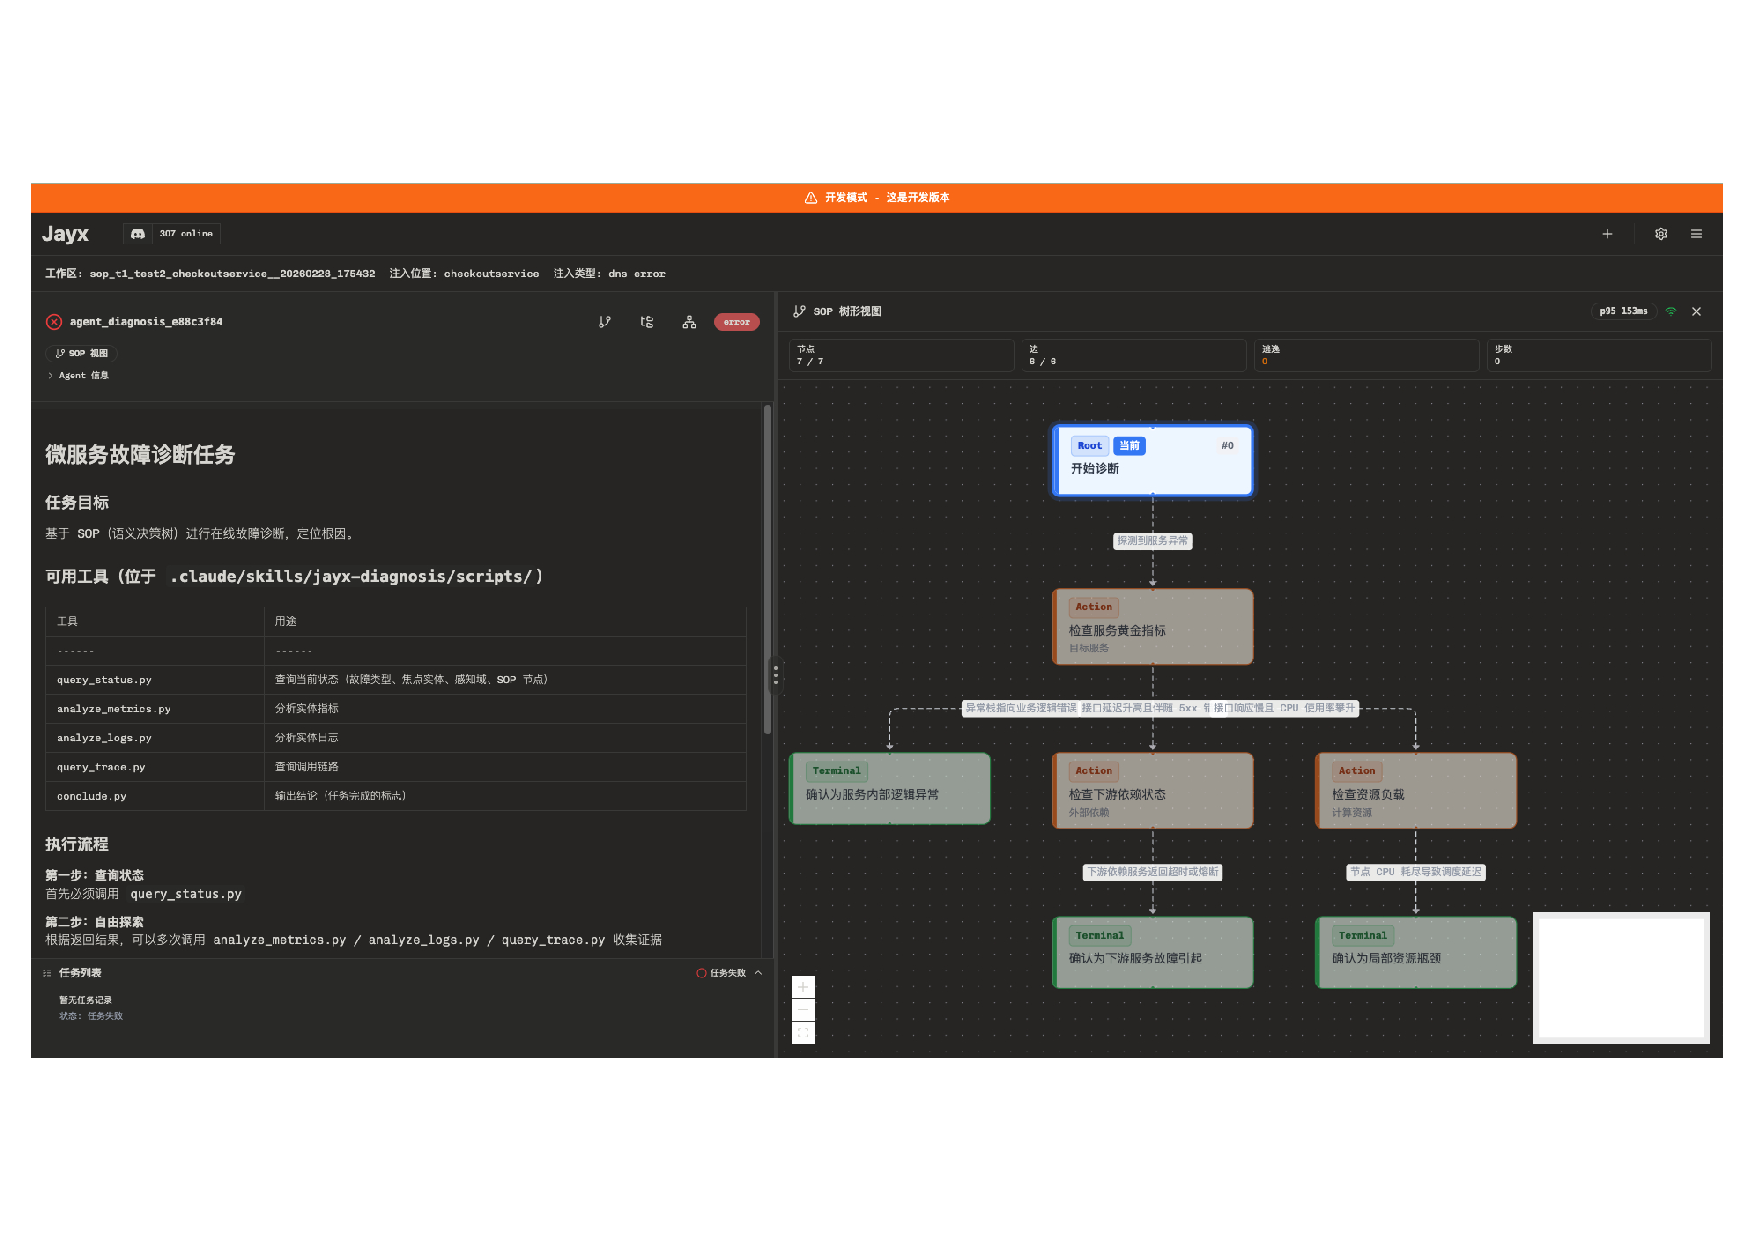
\includegraphics[width=0.96\textwidth]{Figures-Src/Chap4-System/user-interaction/fig1-sop-navigation.pdf}
    \bicaption{\enspace 诊断执行界面：左侧为 Agent 诊断日志与任务进度，右侧为 SOP 节点图}{\enspace Diagnosis Execution Interface: Left shows Agent diagnosis log and task progress, right shows SOP node graph}
    \label{fig:user_sop_navigation}
\end{figure}
\FloatBarrier

该界面用于将在线诊断过程与 SOP 路径状态对应起来。左侧消息区记录任务推进过程、工具返回结果和阶段性结论，右侧节点图同步标示当前节点及已执行路径。通过这一界面，用户不仅能够观察系统是否沿既有 SOP 持续推进，还能够识别其是否已经暂时脱离当前 SOP 并进入探索分支，从而更直观地理解诊断过程的演化状态。

\clearpage

\subsection{工作区界面}

工作区界面是案例级任务的统一入口，同时承载第 3.3 节对应的离线知识构建任务和在线诊断任务。如图\ref{fig:user_workspace}所示，每个工作区绑定一个具体案例。页面顶部展示工作区名称、注入位置和注入类型，中部以任务卡片形式展示该案例下的各类任务，并按照任务状态和任务类型进行分类。

\begin{figure}[htbp]
    \centering
    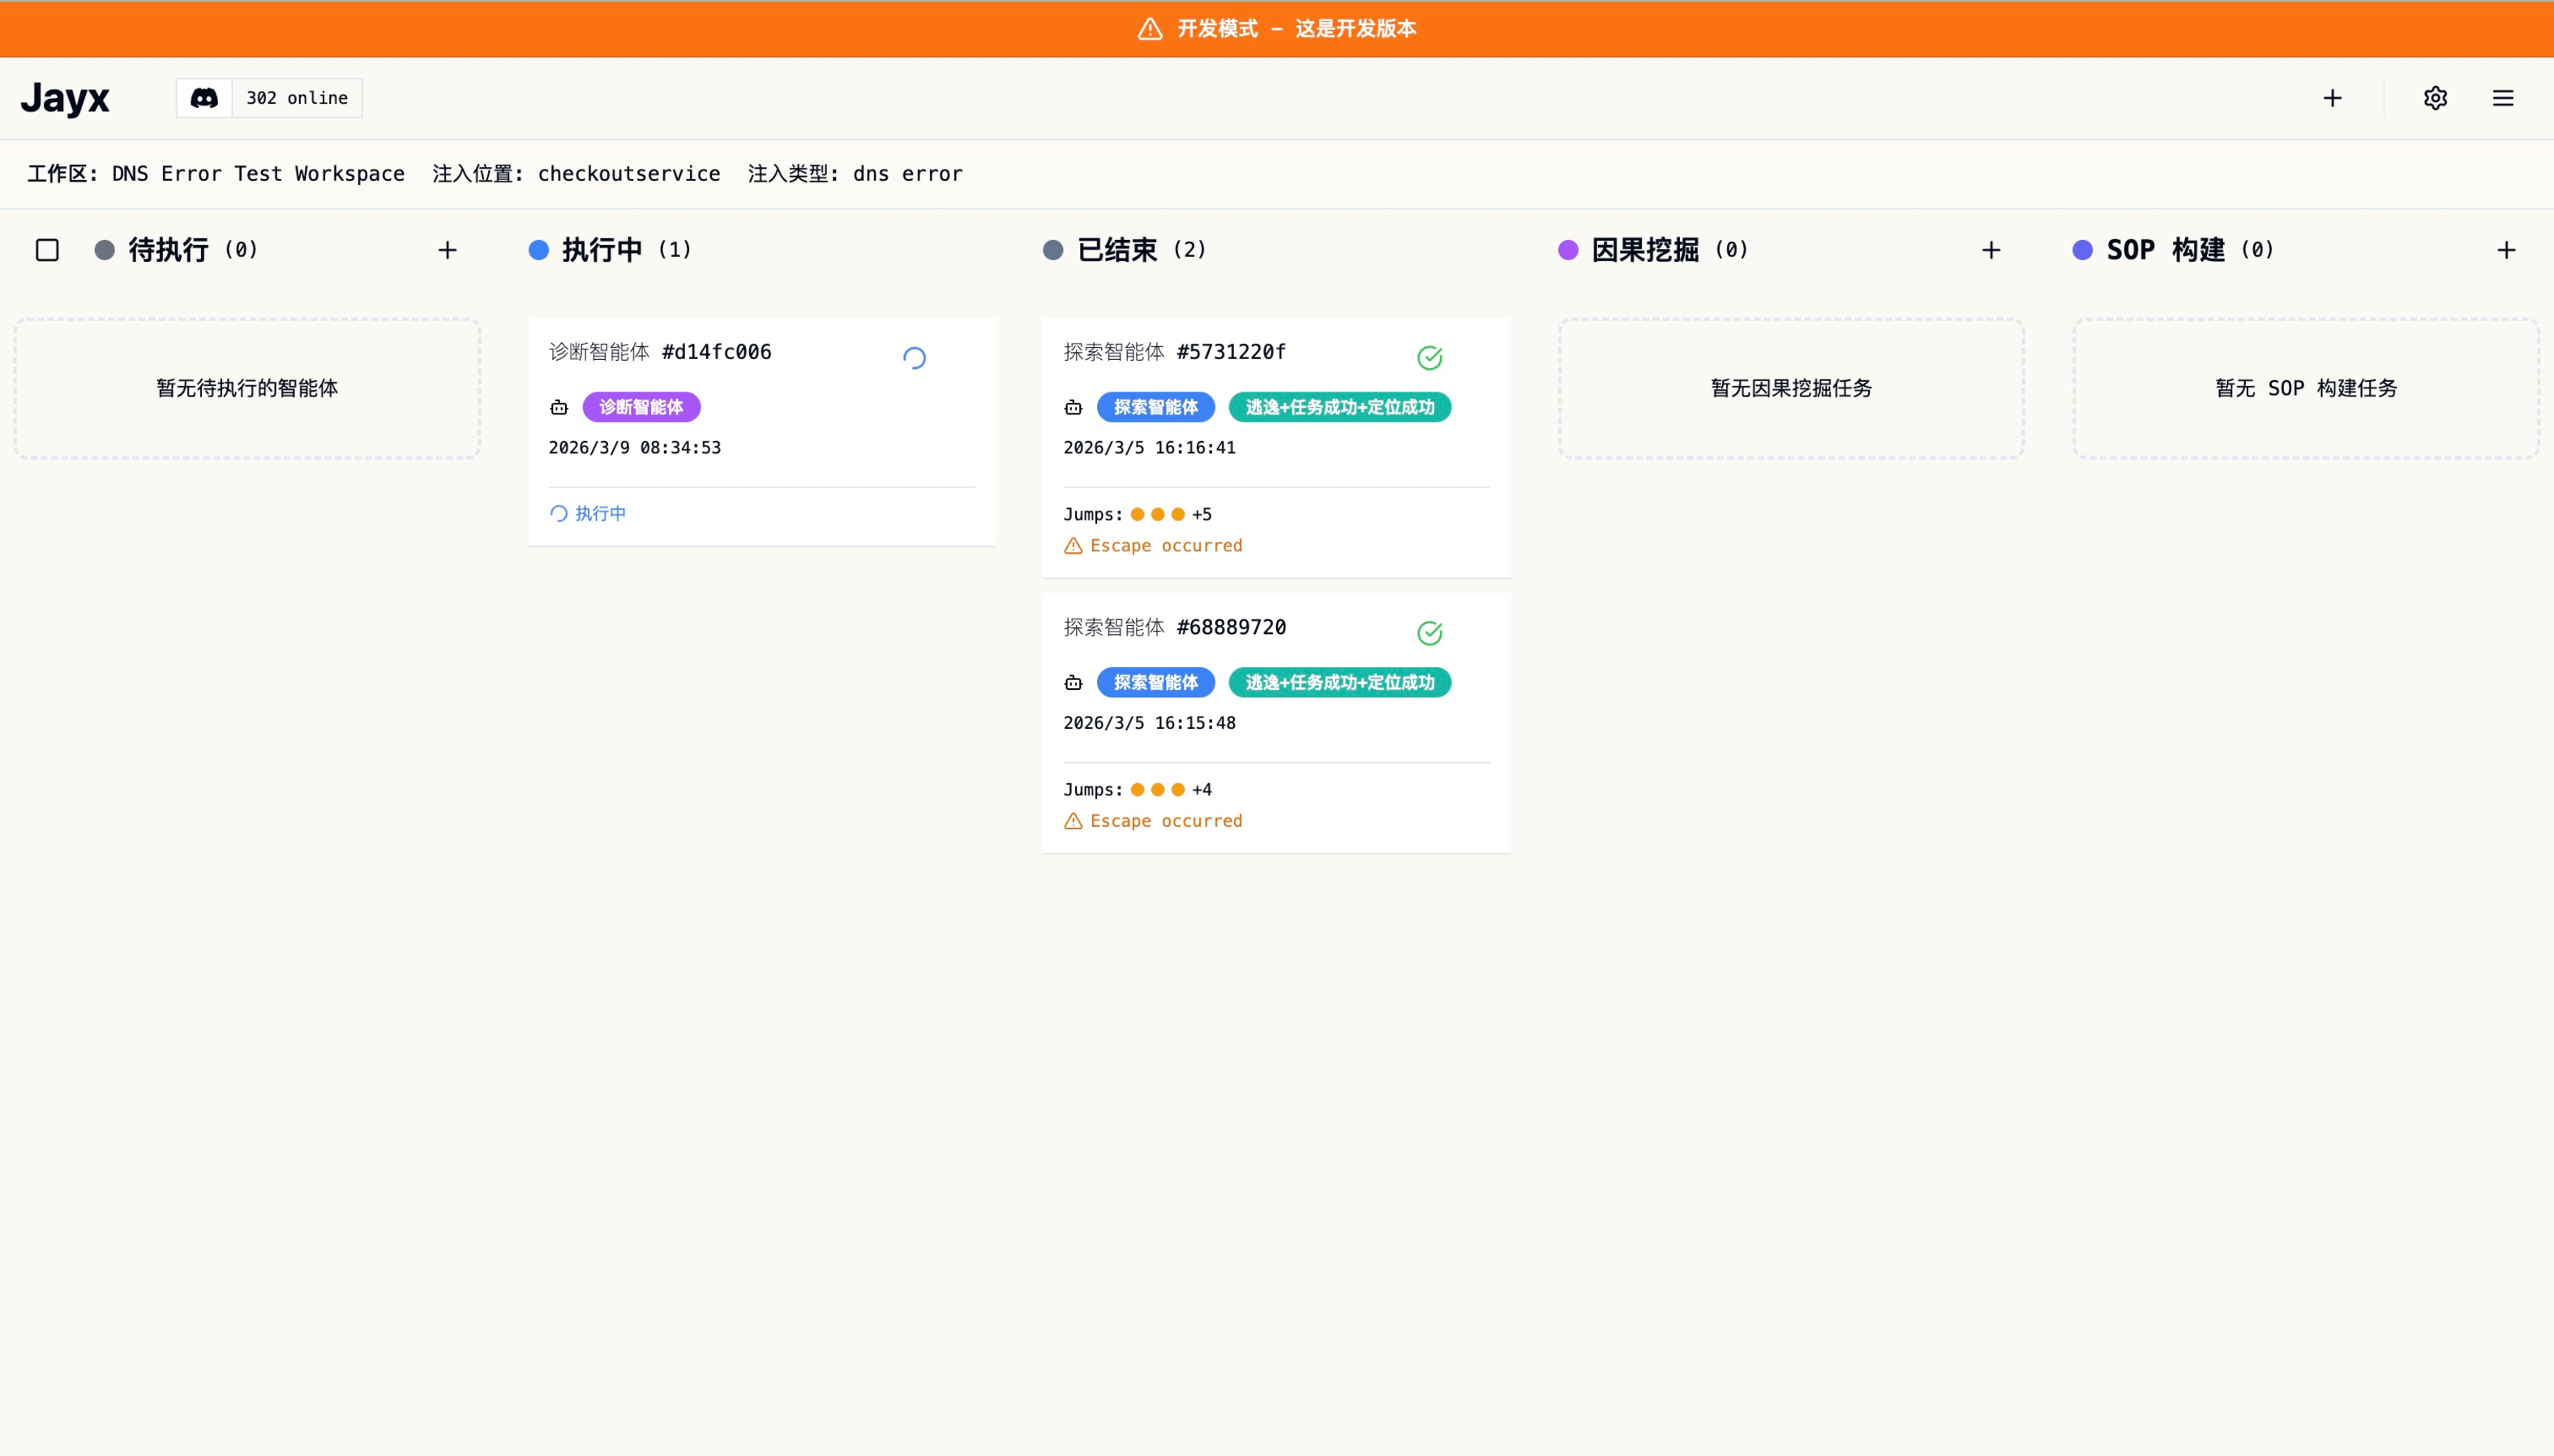
\includegraphics[width=0.96\textwidth]{Figures-Src/Chap4-System/user-interaction/fig2-workspace.pdf}
    \bicaption{\enspace 工作区中的案例信息与任务看板}{\enspace Case Context and Task Board in the Workspace}
    \label{fig:user_workspace}
\end{figure}
\FloatBarrier

工作区界面将同一案例相关的任务与中间结果组织在统一上下文下。在该界面中，用户可以创建诊断任务、探索任务、挖掘任务和 SOP 构建任务，也可以查看各任务对应的执行状态与输出结果。诊断结论、SOP 执行轨迹、决策单元提取结果以及 SOP 更新结果均保存在同一工作区内，便于围绕单个案例持续跟踪、回溯和管理。

\clearpage

\subsection{故障指纹界面}

故障指纹界面用于展示故障指纹库中的聚类结果及其样本分布。如图\ref{fig:user_fingerprint_3d}所示，系统采用 t-分布随机邻域嵌入（t-distributed Stochastic Neighbor Embedding，t-SNE）方法，将高维故障指纹投影到三维空间。界面左侧列表展示各聚类的编号、样本数和代表标签，右侧散点图展示样本在三维嵌入空间中的分布。

\begin{figure}[htbp]
    \centering
    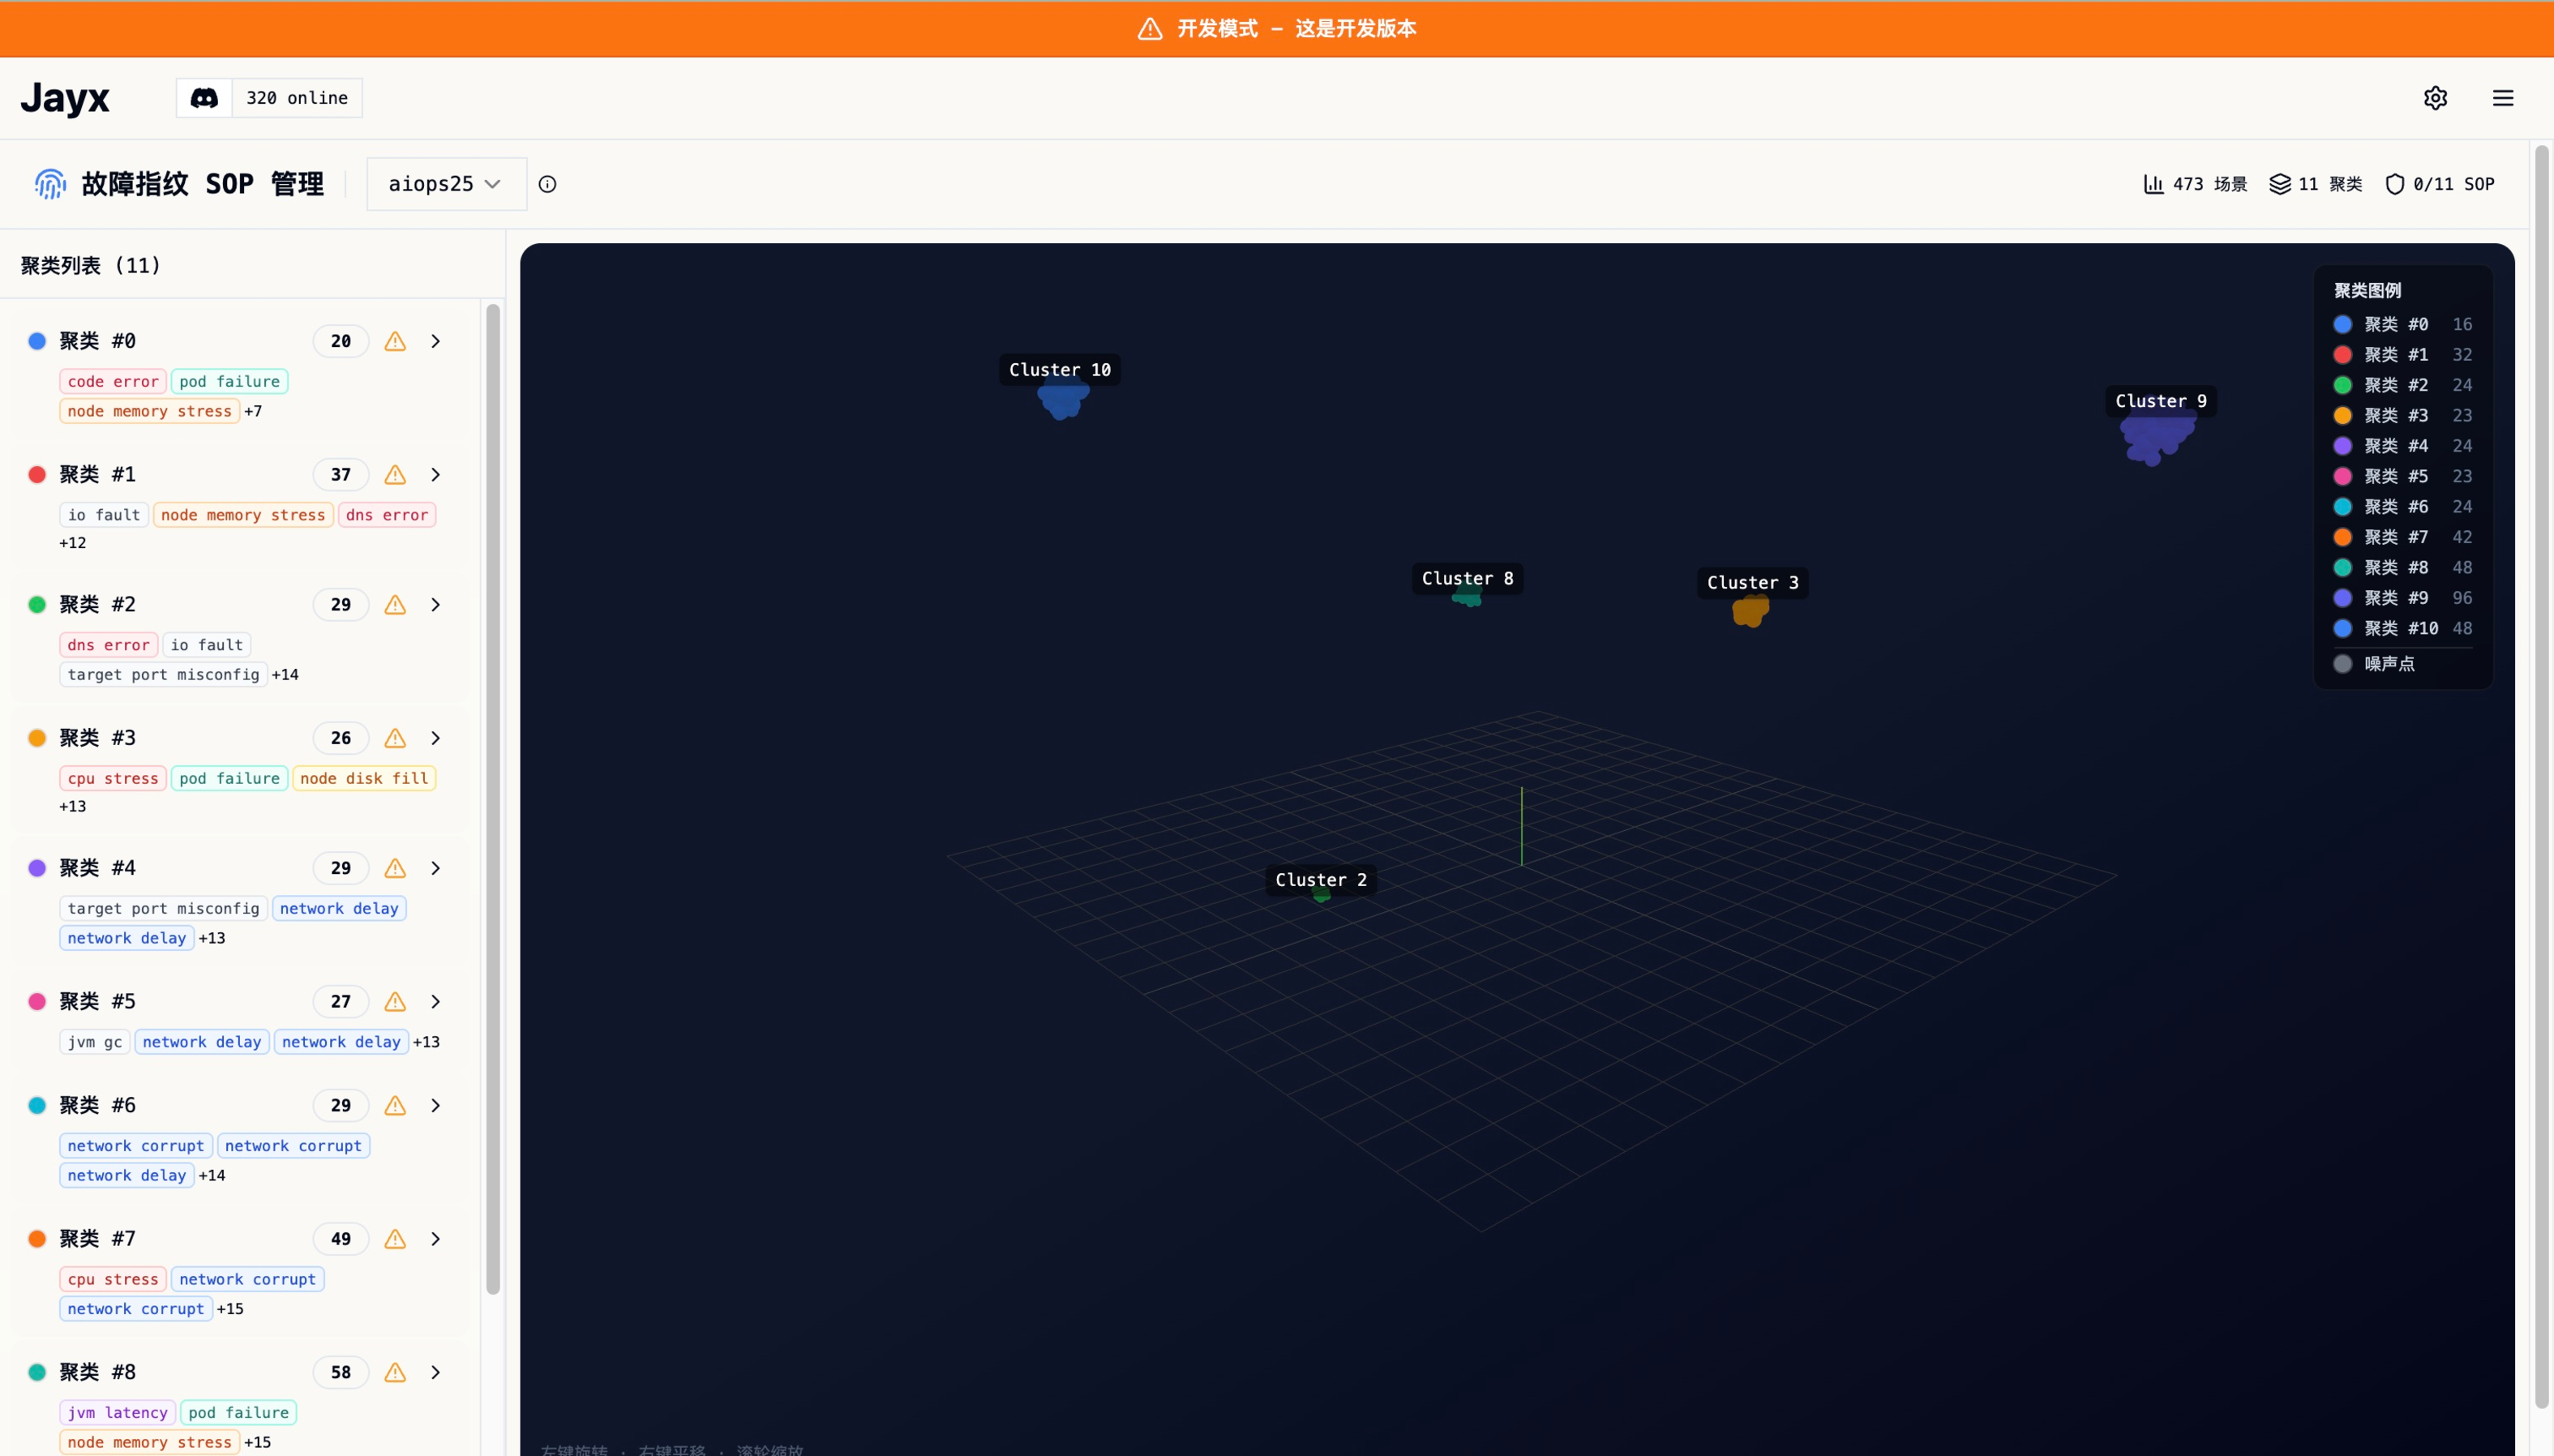
\includegraphics[width=0.96\textwidth]{Figures-Src/Chap4-System/user-interaction/fig3-fingerprint-3d.pdf}
    \bicaption{\enspace 三维嵌入空间中的故障指纹聚类分布}{\enspace Fault Fingerprint Clusters in a 3D Embedding Space}
    \label{fig:user_fingerprint_3d}
\end{figure}
\FloatBarrier

图中每个点对应一个故障实例，颜色表示其所属聚类。用户可以通过该界面定位特定聚类，查看其代表标签、样本规模和空间分布，并结合实例信息检查故障指纹库中的聚类结果。该界面主要用于故障指纹知识的展示与分析，为故障簇分布观察、聚类结果验证和相似故障关系理解提供辅助支持。

综上，诊断执行界面主要用于展示在线诊断过程及其对应的 SOP 路径状态，工作区界面主要用于组织案例级任务及其中间结果，故障指纹界面主要用于查看故障指纹库中的聚类结果与样本分布。三类界面分别服务于任务执行、任务管理与知识查看，共同构成了平台面向用户的主要交互界面。

%---------------------------------------------------------------------------%
%->> 4.5 本章小结
%---------------------------------------------------------------------------%
%------------%
%->> Section 4.5: 本章小结
%--------%

\section{本章小结}

本章围绕故障诊断智能体平台的设计与实现，说明了第三章所提出方法在系统中的落地方式。首先，本文给出了平台的总体架构，说明了前端展示层、Agent 执行层、Skill 组织层、MCP 接入层、后端服务层和数据存储层之间的分工关系，并解释了以 OpenCode 作为执行核心的原因。其次，本文分别说明了故障指纹构建、SOP 自动化构建和在线故障诊断三类方法在平台中的实现位置及其对应的数据流。随后，围绕工作区、任务实体和知识对象，给出了在线诊断任务与离线知识构建任务的执行过程和数据管理方式。最后，本文介绍了诊断执行界面、工作区界面和故障指纹界面，说明了平台如何支持诊断过程展示、案例级任务管理和故障指纹知识查看。

通过上述设计，第三章提出的故障指纹检索、SOP 增量更新和在线诊断执行被组织到同一平台之中，并通过工作区和结果写回机制形成闭环。第五章将在此基础上开展实验验证与分析。
